\documentclass[twoside]{article}

\usepackage{epsfig}
\usepackage{tikz}

\setlength{\oddsidemargin}{0.25 in}
\setlength{\evensidemargin}{-0.25 in}
\setlength{\topmargin}{-0.6 in}
\setlength{\textwidth}{6.5 in}
\setlength{\textheight}{8.5 in}
\setlength{\headsep}{0.75 in}
\setlength{\parindent}{0 in}
\setlength{\parskip}{0.1 in}

\newcommand{\lecture}[4]{
   \pagestyle{myheadings}
   \thispagestyle{plain}
   \newpage
   \setcounter{page}{1}
   \noindent
   \begin{center}
   \framebox{
      \vbox{\vspace{2mm}
    \hbox to 6.28in { {\bf STA561:~Probabilistic machine learning \hfill} }
       \vspace{6mm}
       \hbox to 6.28in { {\Large \hfill #1 (#2)  \hfill} }
       \vspace{6mm}
       \hbox to 6.28in { {\it Lecturer: #3 \hfill Scribes: #4} }
      \vspace{2mm}}
   }
   \end{center}
   \markboth{#1}{#1}
   \vspace*{4mm}
}

\begin{document}

\lecture{Variational Inference}{11/4/13}{Barbara Engelhardt}{Tracy Schifeling, Alireza Samany, and Matt Dickenson}

\section{Introduction}


\section{Ising Model}

% previous section should end with a discussion of ELBO
Before proceeding with variational inference, it is helpful to review the Ising model. The main idea behind the Ising model is a lattice of unobserved variables ($x_1,...x_n$), each with its own (noisy) observation ($y_1, ..., y_n)$). For example, we can think of the lattice as pixels in a black and white image ($x_i \in \{-1, 1\}$), with a noisy grayscale observation of the pixels ($y_i \in R)$. Our goal in this case would be to obtain a de-noised version of the image. More generally, we wish to draw inferences about the unobserved lattice $X$ from the observed values $Y$.

\begin{tikzpicture}
\scriptsize
\foreach \i in {1,...,9}
{
        \pgfmathtruncatemacro{\y}{(\i - 1) / 3};
        \pgfmathtruncatemacro{\x}{\i - 3 * \y};
        \pgfmathtruncatemacro{\label}{\x + 3 * (2 - \y)};
        \pgfmathtruncatemacro{\labely}{(\x + 3 * (2 - \y))*10};
        \node[circle,draw=black,fill=white,minimum size=20]
        (\label) at (1.5*\x,1.5*\y) {$x_\label$};
        \node[circle,draw=black,fill=white!80!black,minimum size=20]
        (\labely) at (1.5*\x-0.8,1.5*\y-0.8) {$y_\label$};
}
% Lattice of X's
\draw (1) -- (2);
\draw (1) -- (4);
\draw (2) -- (3);
\draw (2) -- (5);
\draw (3) -- (6);
\draw (4) -- (5);
\draw (4) -- (7);
\draw (5) -- (6);
\draw (5) -- (8);
\draw (6) -- (9);
\draw (7) -- (8);
\draw (8) -- (9);
% X to Y
\draw (1) -- (10);
\draw (2) -- (20);
\draw (3) -- (30);
\draw (4) -- (40);
\draw (5) -- (50);
\draw (6) -- (60);
\draw (7) -- (70);
\draw (8) -- (80);
\draw (9) -- (90);
% http://tex.stackexchange.com/questions/61805/tikz-using-loop-to-draw-grid-of-nodes
\end{tikzpicture} 


\section{Loopy Belief Propogation}



\end{document}

